\documentclass{scrreprt}
\usepackage{listings}
\usepackage{underscore}
\usepackage[bookmarks=true]{hyperref}
\usepackage[utf8]{inputenc}
\usepackage[english]{babel}
\usepackage{enumitem}
\usepackage{graphicx}
\graphicspath{{work_packages/work_package_1/static/srs/}}
% \graphicspath{{static/srs/}}
\hypersetup{
    pdftitle={Software Requirement Specification},    % title
    pdfauthor={Training Montage},                     % author
    pdfsubject={TeX and LaTeX},                        % subject of the document
    pdfkeywords={TeX, LaTeX, graphics, images}, % list of keywords
    colorlinks=true,       % false: boxed links; true: colored links
    linkcolor=blue,       % color of internal links
    citecolor=black,       % color of links to bibliography
    filecolor=black,        % color of file links
    urlcolor=purple,        % color of external links
    linktoc=page            % only page is linked
}

\def\myversion{0.1 }
\date{}

\usepackage{hyperref}
\begin{document}

\begin{flushright}
    \rule{16cm}{5pt}\vskip1cm
    \begin{bfseries}
        \Huge{SOFTWARE REQUIREMENTS\\ SPECIFICATION}\\
        \vspace{.9cm}
        for\\
        \vspace{.9cm}
        COE 1186 Project\\
        \vspace{.9cm}
        \LARGE{Version \myversion approved}\\
        \vspace{.9cm}
        Prepared by:\\
        Alec Rosenbaum\\
        Aric Hudson\\
        Isaac Goss\\
        Mitch Moran\\
        Parth Dadhania\\
        \vspace{1.9cm}
        Training Montage\\
        \vspace{.9cm}
        \today\\
    \end{bfseries}
\end{flushright}

\tableofcontents

\chapter*{Revision History}

\begin{center}
    \begin{tabular}{|c|c|c|c|}
        \hline
	    Name & Date & Reason For Changes & Version\\
        \hline
        et all & September 24, 2017 & Module Requirements & 0.2.0\\
        \hline
	    Alec Rosenbaum & September 14, 2017 & init & 0.1\\
        % \hline
	    % 31 & 32 & 33 & 34\\
        \hline
    \end{tabular}
\end{center}

\chapter{Introduction}

\section{Purpose}
The product whose software requirements are specified in this document is the
Training Montage Rail Simulator (TMRS). This SRS covers the functional and
non-functional requirements, design constraints, and functional limitations that
will be observed during the development of this project. This SRS will encompass
the entire system, and will include specific requirements, constraints, and
limitations for each sub-system.

\section{Document Conventions}
The following acronyms will be used throughout the paper:

\begin{description}
  \item[TMRS] Training Montage Rail Simulator
  \item[Failure] A subsystem has failed when it allows two locomotives to share a block.
  \item[Unsafe] A situation or subsystem is unsafe if failure is made possible by said situation or subsystem.
  \item[Vital] A vital subsystem is one which shall not allow unsafe output.
  \item[PLC] Programmable Logic Controller, a hardware platform which operates solely on binary values, controlled by code given by a user. The term PLC will be used interchangeably to refer to the device and the code which runs on it.
  \item[CTC] Centralized Traffic Control, the module that represents the main dispatcher office.
  \item[Block] The track is partitioned into blocks, what is considered an indivisible unit of track. A block has one speed limit, one grade, one altitude, no switches, and at most one train occupying it.
\end{description}

\section{Intended Audience and Reading Suggestions}
This document is intended as a part of the contractual agreement between Training
Montage and their client for the TMRS software package. It will be used as reference
by developers, project managers, testers, and the client.

It is suggested that the user read over the project scope and perspective, then
visit the UI design prototype included in the Appendix. The UI design prototype
will give a good sense of how users will interact with the software, and of what
capabilities are provided by the system. After reviewing the UI design prototype,
proceed to read the rest of the document in the order that it's presented.

\section{Project Scope}
This project shall have many deliverables, organized into three Work Packages (WPs).

\begin{enumerate}[label=\textbf{WP \arabic*.}]
    \item This includes project planning and requirement gathering, due Thursday, September 28, 2017.
    It will contain the following deliverables:
    \begin{enumerate}
        \item The Software Requirements Specification, this very document.
        \item User Interface prototype.
        \item User's Manual detailing the functionality of the aforementioned UI.
        \item Risk Assessment.
        \item Coding Standard.
        \item Defect Tracking Policy.
        \item Schedule detailing our expected progress.
    \end{enumerate}

    \item This is the phase in which the system shall be designed, due Thursday, November 2, 2017.
    \begin{enumerate}
        \item System Architecture and Design.
        \item Test Plan.
        \item Updated Schedule with resource assignments.
    \end{enumerate}

    \item This is the implementation phase. The requirements and design will be implemented to create a working system, due Thursday, September 7, 2017.
    \begin{enumerate}
        \item Code Base of the implemented application.
        \item Installation Guide.
        \item Configuration Management.
        \item Executed Test Plan.
        \item Defect Reports.
        \item Project Presentation.
    \end{enumerate}
\end{enumerate}

%\section{References}
%$<$ TBD $>$

\chapter{Overall Description}

\section{Product Perspective}
TMRS is a simulation and prototype bid for the North Shore Extension presented by the City of Pittsburgh, PA.
In this capacity, the software is intended to allow users view of how a completed North Shore Extension control system would operate, and serve to inform the development of the system to be deployed, although no code will be shared between this prototype and the completed system.

There are five major modules which make up this system, for which the individual requirements will be specified in chapter 4.

\begin{description}
    \item[Centralized Traffic Control (CTC)] The CTC office module is the part of the software that sends trains from the train yard.
    A human dispatcher can view information of the entire system from the CTC office.
    The module can operate in automatic mode, where it dispatches and routes trains according to a set schedule, or manual mode where trains are dispatched by the dispatcher.
    \item[Wayside / Track Controller] This module is a vital computing platform.
    The Wayside Controller module is a simulation of the many wayside controllers which sit next to track, and operate the switches and lights on the track, and provide the train traveling with within its region safe speed and authority.
    \item[Track Model] The system shall have a model of the transit system track layout. This module is \textbf{not} vital.
    \item[Train Model] The Train Model models the movement of the train using Newton's laws of motion
    assuming that the train is a rigid body point mass. This is a non-vital module.
    \item[Train Controller] This module is responsible for safely dictating the train's speed by way of controlling its power, as well as controlling some smaller tasks like light and door control, and feedback about current and approaching stations. This module is VITAL.
\end{description}


%$<$Describe the context and origin of the product being specified in this SRS.
%For example, state whether this product is a follow-on member of a product
%family, a replacement for certain existing systems, or a new, self-contained
%product. If the SRS defines a component of a larger system, relate the
%requirements of the larger system to the functionality of this software and
%identify interfaces between the two. A simple diagram that shows the major
%components of the overall system, subsystem interconnections, and external
%interfaces can be helpful.$>$

\section{Product Functions}
The software shall:
    \begin{enumerate}
        \item Allow a dispatcher to perform tasks such as create, view, edit, and execute schedules, and also manually dispatch a train to a location.
        \item Allow a wayside engineer to control the operation of switches and lights with PLC code.
        \item Allow a locomotive engineer to observe automatic train operation, and also allow manual train control.
        \item Move trains to their destination always in a SAFE manner.
    \end{enumerate}

\section{User Classes and Characteristics}
This produce is expected to be used by the following classes of users:
\begin{enumerate}
    \item Dispatcher
    \item Wayside Engineer
    \item Train Conductor
\end{enumerate}

It is expected none of these user classes to have technical expertise. As such,
each user will be provided with an graphical user interface that allows full
functionality of each module.

It is, however, expected that Wayside Engineers are experts both on a section
of track and in writing PLC code. All uploaded code is considered vital.

\section{Operating Environment}
The software will operate on the Java Virtual Machine. The Java Virtual Machine
can be installed on computers with a Pentium 2 266 MHz or faster processor, at
least 128 MB of physical RAM, and 124MB of free disk space. Java supports Windows,
Mac OS X, Linux, and Solaris. We will be writing software using Java Version 8.
This software shall be executable on Windows 10 operating system.

\section{Design and Implementation Constraints}
\begin{enumerate}
    \item The Wayside Controller is a PLC, meaning that it can only operate on simple binary values. Any PLC code written for it shall observe this constraint.
\end{enumerate}
%$<$Describe any items or issues that will limit the options available to the
%developers. These might include: corporate or regulatory policies; hardware
%limitations (timing requirements, memory requirements); interfaces to other
%applications; specific technologies, tools, and databases to be used; parallel
%operations; language requirements; communications protocols; security
%considerations; design conventions or programming standards (for example, if the
%customer’s organization will be responsible for maintaining the delivered
%software).$>$

\section{User Documentation}

The following documentation components will be delivered along with the software:
\begin{enumerate}
    \item UI Design
    \item User's Manual
\end{enumerate}

\section{Assumptions and Dependencies}
It is assumed that every user has a static map of the track detailing block information.
%$<$List any assumed factors (as opposed to known facts) that could affect the
%requirements stated in the SRS. These could include third-party or commercial
%components that you plan to use, issues around the development or operating
%environment, or constraints. The project could be affected if these assumptions
%are incorrect, are not shared, or change. Also identify any dependencies the
%project has on external factors, such as software components that you intend to
%reuse from another project, unless they are already documented elsewhere (for
%example, in the vision and scope document or the project plan).$>$


\chapter{External Interface Requirements}

\section{User Interfaces}
There will a be discrete user interface for each System Module. These user
interfaces will be capable of running separately, but may also be run together
in order to show the full functionality of each module and how it interfaces
behind-the-scenes with other modules.

UI Prototypes for each module are shown in the UI Design document. The User's
Manual further elaborates on operational details and how users are expected to
interface with each module.


%
%$<$Describe the logical characteristics of each interface between the software
%product and the users. This may include sample screen images, any GUI standards
%or product family style guides that are to be followed, screen layout
%constraints, standard buttons and functions (e.g., help) that will appear on
%every screen, keyboard shortcuts, error message display standards, and so on.
%Define the software components for which a user interface is needed. Details of
%the user interface design should be documented in a separate user interface
%specification.$>$

%\section{Hardware Interfaces}
%$<$Describe the logical and physical characteristics of each interface between
%the software product and the hardware components of the system. This may include
%the supported device types, the nature of the data and control interactions
%between the software and the hardware, and communication protocols to be
%used.$>$

%\section{Software Interfaces}
%    The software shall interface with the Java Virtual Machine version 8, and the Windows 10 operating system.

%$<$Describe the connections between this product and other specific software
%components (name and version), including databases, operating systems, tools,
%libraries, and integrated commercial components. Identify the data items or
%messages coming into the system and going out and describe the purpose of each.
%Describe the services needed and the nature of communications. Refer to
%documents that describe detailed application programming interface protocols.
%Identify data that will be shared across software components. If the data
%sharing mechanism must be implemented in a specific way (for example, use of a
%global data area in a multitasking operating system), specify this as an
%implementation constraint.$>$

%\section{Communications Interfaces}
%$<$Describe the requirements associated with any communications functions
%required by this product, including e-mail, web browser, network server
%communications protocols, electronic forms, and so on. Define any pertinent
%message formatting. Identify any communication standards that will be used, such
%as FTP or HTTP. Specify any communication security or encryption issues, data
%transfer rates, and synchronization mechanisms.$>$


\chapter{System Modules}
This application shall be made of 5 separate modules, each of which a team member shall own.
These shall be the Centralized Traffic Controller, Wayside / Track Controller, Track Model, Train Model, and Train Controller.
These modules shall have strict communication constraints and be organized in the following way.

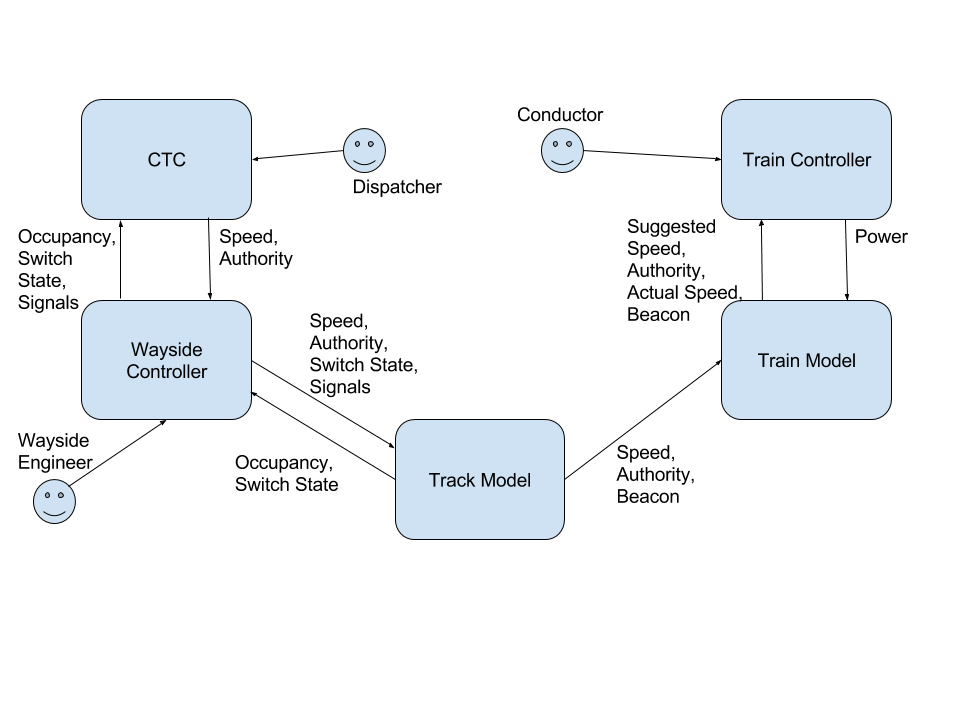
\includegraphics[width=\textwidth]{srs-module-overview}

\section{Centralized Traffic Control (CTC) Office Module}

\subsection{Description}
The CTC office module is the part of the software that sends trains from the
train yard. A human dispatcher can view information of the entire system
from the CTC office. The module can operate in automatic mode, where is dispatches
and routes trains according to a set schedule, or manual mode where trains are
dispatched by the dispatcher.

\subsection{Interface}
The CTC module interacts with two users, a human dispatcher and the wayside controller
module.
\begin{enumerate}
    \item The module must display information on the current track layout and currently
    deployed trains to the dispatcher.
    \item The dispatcher can manually schedule trains for the CTC to deploy.
\end{enumerate}
\begin{enumerate}
    \item The CTC gives suggested speed and authority for each train to the wayside
    controller module.
    \item The wayside controller module will send the CTC information on which pieces of
    track are occupied by trains.
\end{enumerate}
There is also a communication link between the stations of the track model and the
CTC to communicate information on passenger throughput.

\subsection{Functional Requirements}
\begin{enumerate}
    \item The CTC module must display the following track information. Some information
    will be displayed in a dynamic map view and detailed information will be displayed
    when selecting a block in the map view. Items indicated with an asterisk (*) are only 
    displayed when relevant. 
    \begin{enumerate}
        \item Block ID
        \item Block Region
        \item Occupied State
        \item Speed Limit
        \item Length
        \item Grade
        \item Elevation
        \item Block Passable (Yes, Broken, or Maintenance)
        \item Heater (On, Disabled, N/A)
        \item Underground/Above Ground
        \item Light Information* 
        \begin{enumerate}
            \item Light State (Super Green, Green, Yellow, Red)
        \end{enumerate}
        \item Switch Information* 
        \begin{enumerate}
            \item Switch ID
            \item Switch State
        \end{enumerate}
        \item Station Information* 
        \begin{enumerate}
            \item Station Name
            \item Number of Passengers
        \end{enumerate}
        \item Railway Crossing*
        \begin{enumerate}
          \item Activated
        \end{enumerate}
    \end{enumerate}
    \item The CTC module must let the dispatcher close and open blocks for maintenance.
    \item The CTC module must be able to operate in manual or automatic mode. In manual
    mode, all trains will be manually dispatched by the human dispatcher. In automatic
    mode, trains will be dispatched by the module according to a schedule.
    \item The CTC module must let the dispatcher upload a schedule to be followed in
    automatic mode.
    \item The CTC module must let the dispatcher view and edit the schedule in manual mode.
    \item The CTC module must display the following train information. Some information
    will be displayed in a dynamic map view and detailed information will be displayed
    when selecting a train in the map view.
    \begin{enumerate}
        \item Train ID
        \item Current Block
        \item Suggested Speed
        \item Given Authority
        \item Origin
        \item Destination
    \end{enumerate}
    \item The CTC module must display the ambient temperature.
    \item The CTC module must display the current passenger throughput based on tickets
    sold at each station.
\end{enumerate}


\section{Wayside / Track Controller}

\subsection{Description}
This module is a vital computing platform.
The Wayside Controller module is a simulation of the many wayside controllers which sit next to track, and operate the switches and lights on the track, and provide the train traveling with within its region safe speed and authority.

\subsection{Interface}
\begin{enumerate}
    \item The Wayside Controller shall accept suggested (non-vital) speed and authority (per train) from the CTC.
    \item The Wayside Controller shall accept block occupancy and switch positions from the Track Model.
    \item The Wayside Controller shall have vital outputs to the Track Model:
    \begin{enumerate}
        \item Speed \& Authority per train.
        \item Light colors per track block.
        \item Switch positions.
        \item Railway crossings.
    \end{enumerate}
    \item The Wayside Controller shall report the following back to the CTC:
    \begin{enumerate}
        \item Broken rail.
        \item Railway crossings.
        \item Block occupancy.
        \item Switch positions.
        \item Light colors.
    \end{enumerate}
\end{enumerate}

\subsection{Functional Requirements}
\begin{enumerate}
    \item The Wayside Controller shall be a vital computing platform.
    \item The Wayside Controller shall receive suggested speed and authority from the CTC per train, and output safe speed and authority per train.
    \item The Wayside Controller shall control the switching of the track.
    \item The Wayside Controller shall detect broken blocks of rail.
    \item The Wayside Controller shall report the state of the track, railway crossings, signals, and occupancy to the CTC.
    \item This is a PLC, and shall allow a user, a Wayside Engineer, to upload a code to control it. It is assumed that this Wayside Engineer's code is vital. The implementation of this shall be diverse.
\end{enumerate}



\section{Track Model}

\subsection{Description}
The system shall have a model of the transit system track layout. This module is not VITAL.

\subsection{Interface}
\begin{enumerate}
    \item The Track Model shall accept speed and authority as inputs from the Wayside Controller.
    \item The Track Model shall provide block occupancy and switch positions to the Wayside Controller.
    \item The Track Model shall provide speed and authority to the Train Model.
\end{enumerate}

\subsection{Functional Requirements}
\begin{enumerate}
    \item The Track Model shall consider grade and elevation.
    \item The Track Model shall be configurable.
    \item The Track Model shall consider allowable directions of travel, branching, and speed limits.
    \item The Track Model shall be able to export and import track layouts.
    \item The Track Model shall consider block size.
    \begin{enumerate}
        \item Blocks must be shown and configurable.
    \end{enumerate}
    \item The Track Model shall signals and switch machines.
    \item The Track Model shall implement track circuits for presence detection.
    \item The Track Model shall consider railway crossings.
    \item The Track Model shall include stations.
    \begin{enumerate}
        \item Passengers shall be loaded and unloaded at stations.
    \end{enumerate}
    \item The Track Model shall implement the following failure modes:
    \begin{enumerate}
        \item Broken rail
        \item Track Circuit failure
        \item Extra or no trains detected
        \item Power failure
        \item No communication going to train
    \end{enumerate}
\end{enumerate}

\section{Train Model}

\subsection{Description}
The Train Model models the movement of the train using Newton's laws of motion
assuming that the train is a rigid body point mass. This is a non-vital module.

\subsection{Interface}
The Train Model shall take in speed and authority from Track Model. It shall
output the speed and authority to the Train Controller.

\subsection{Functional Requirements}
\begin{enumerate}
  \item Train Specifications
   \begin{enumerate}
    \item Length
    \item Height
    \item Width
    \item Mass
    \item Passenger Count
    \item Crew Count
   \end{enumerate}
  \item Physics/Inputs
  \begin{enumerate}
   \item Authority
   \item Speed Limit
   \item Acceleration/Deceleration Limit
   \item Door open/close
   \item Lights on/off
   \item Temperature Control
   \item Emergency Brake
   \item Brake Command
   \item Setpoint Speed Command
   \item Track Circuit
   \item Transponder
   \item Route Information System
  \end{enumerate}
  \item Failure Modes
    \begin{enumerate}
     \item Brake Failure
     \item Signal Pickup Failure
     \item Train Engine Failure
    \end{enumerate}
\end{enumerate}


\section{Train Controller}

\subsection{Description}
This module is responsible for safely dictating the train's speed by way of controlling its power, as well as controlling some smaller tasks like light and door control, and feedback about current and approaching stations. This module is VITAL.

This vital controller receives a suggested speed and compares it to its own calculated maximum safe speed and selects the lower of the two values to relay to the Train Model. As the train's speed is controlled by its current power, the Train Controller converts the new speed into a power requirement (or a brake setting, if needed).  The train controller also dictates when the lights and doors should be activated, and announces when the train is approaching a station or has stopped at a station.

\subsection{Interface}
The Train Controller receives a suggested speed from the Wayside Controller. This information will be processed and relayed to the Train Model as a power setting.  The controller sends signals to turn lights on or off, and open doors on either side of the train.  This module receives feedback from the Train Model in the from of its current speed and/or power.  The Train Controller also knows the train's current authority in the form of distance in miles.

\subsection{Functional Requirements}
\begin{enumerate}
    \item The Train Controller shall have an algorithm capable of calculating a maximum safe speed for the train in question.
    \begin{enumerate}
        \item The maximum safe speed shall be the maximum speed that can be fully arrested in the minimum safe breaking distance.
        \item The train controller shall consider the train's mass, current speed, and current authority when calculating this speed.
    \end{enumerate}

    \item The Train Controller shall select a safe speed for the train.
    \begin{enumerate}
        \item The Train Controller shall choose the suggested speed or its own calculated maximum safe speed.
        \item By default, the lower of the two speeds will be chosen for the train.
        \item The Train Controller shall allow a manual mode for the driver of the train to manually input a speed.  This speed shall not exceed the speed suggested by the Wayside Controller.
    \end{enumerate}

    \item The module, once it has chosen a speed for the train, will require an algorithm to convert that desired speed into either (1) a power setting for the train, or (2) an application of the brake for a certain amount of time.
    \begin{enumerate}
        \item This algorithm shall use the train's current and desired kinetic energy combined with a time constraint to determine the power required to achieve the desired speed.
        \item This algorithm shall also take grade into account.
        \item The details of this algorithm are TBD.
    \end{enumerate}

    \item The Train Controller must dictate that lights should be turned on or off.
    \begin{enumerate}
        \item The Train Controller shall control lights based on a daily schedule.
        \item It is the responsibility of the Train Model to execute these instructions.
    \end{enumerate}

    \item The Train Controller must dictate that train doors should open.
    \begin{enumerate}
        \item The Train Controller shall only open doors when the train is stopped.
        \item Doors can be opened on the left or the right, or both.
        \item The Train Controller shall read which doors should be open from beacons approaching each station.
        \item In the event of an emergency stop and train evacuation, the Train Controller shall send the command to open whichever doors are appropriate, given the situation at hand.
        \item It is the responsibility of the Train Model to execute these instructions.
    \end{enumerate}

    \item The Train Controller must display stops and stations.
    \begin{enumerate}
        \item The upcoming stop and the distance to that stop shall be read from an RFID sensor one block before the station or stop's location.
        \item The Train Controller shall display the stop as soon as it receives and deciphers the information from the RFID sensor.
        \item The Train Controller shall display the information until the train has physically left that station.
    \end{enumerate}
\end{enumerate}

\chapter{Other Nonfunctional Requirements}

\section{Performance Requirements}
The simulation software must be able to simulate at 10 times wall clock speed.
This will allow quicker evaluation of a simulated circumstances. The simulation
speed should be modifiable during simulation; i.e. it specified while the simulation
is running, rather than before the software starts.

\section{Safety Requirements}
No train shall at any point collide with any other train. Trains shall not share blocks. No train shall exceed
the speed limit or authority.
%$<$Specify those requirements that are concerned with possible loss, damage, or
%harm that could result from the use of the product. Define any safeguards or
%actions that must be taken, as well as actions that must be prevented. Refer to
%any external policies or regulations that state safety issues that affect the
%product’s design or use. Define any safety certifications that must be
%satisfied.$>$



%\chapter{Other Requirements}
%$<$Define any other requirements not covered elsewhere in the SRS. This might
%include database requirements, internationalization requirements, legal
%requirements, reuse objectives for the project, and so on. Add any new sections
%that are pertinent to the project.$>$

%\section{Appendix A: Glossary}
%%see https://en.wikibooks.org/wiki/LaTeX/Glossary
%%$<$Define all the terms necessary to properly interpret the SRS, including
%%acronyms and abbreviations. You may wish to build a separate glossary that spans
%%multiple projects or the entire organization, and just include terms specific to
%%a single project in each SRS.$>$

%\section{Appendix B: Analysis Models}
%$<$Optionally, include any pertinent analysis models, such as data flow
%diagrams, class diagrams, state-transition diagrams, or entity-relationship
%diagrams.$>$

%\section{Appendix C: To Be Determined List}
%$<$Collect a numbered list of the TBD (to be determined) references that remain
%in the SRS so they can be tracked to closure.$>$

\end{document}
